\documentclass[paper=a4, fontsize=12bp]{scrreprt}
%Einbinden der ben�tigten Pakete �ber die Datei Pakete.tex, wobei die Dateiendung weggelassen wird
\usepackage[T1]{fontenc}
\usepackage[utf8]{inputenc}
\usepackage{mathptmx}				%Font: Times New Roman
%\usepackage[default]{droidserif}	%Font: Droid Serif
\usepackage[ngerman]{babel}
%Seitenränder einstellen
\usepackage[head=2cm,bottom=2cm, left=25mm, right= 25mm ]{geometry}
%Paket für Erzeugung eines Abkürzungsverzeichnis, über das auch per Befehl im späteren Text auf diese verwiesen werden kann
\usepackage[printonlyused,smaller]{acronym}
%Paket zur Gestaltung der Kopf- und Fusszeile bei KOMA-Script
\usepackage{scrpage2}
\usepackage[hidelinks]{hyperref}
%Bibliograpie Packages / Settings
\usepackage{ragged2e} % Ermöglicht Flattersatz mit Silbentrennung
\usepackage[babel,german=guillemets]{csquotes}
% damit werden Zitate in französische Anführungszeichen gesetzt
\usepackage[%
backend=biber,% damit wird bestimmt, dass Sie mit der biber.exe arbeiten
bibencoding=utf8,% steht für die Kodierung der .bib-Datei
bibwarn=true,% damit werden ggf. enstandene Fehler ausgegeben
style=alphabetic,% hier wird die DIN 1505-T2 eingebunden
%firstinits=true% der Familienname des Authors wird an die erste Stelle
% gesetzt und anschließend der Vorname nur mit dem ersten
% Buchstaben abgekürzt ausgegeben
]{biblatex}
\usepackage[babel]{microtype} % bringt optischen Randausgleich und
% minimale Skalierung der Buchstaben
\setlength\bibitemsep{8pt} % Abstand zwischen 2 Einträgen im Verzeichnis
% nachfolgend wird der Kopf des Literaturverzeichnisses bestimmt
\defbibheading{online}{\subsection*{Online-Quellen}}
\defbibheading{offline}{\subsection*{Literatur}}
\ExecuteBibliographyOptions{
%isbn=false, % falls die ISBN hinterlegt ist wird diese ausgeblendet
}
\addbibresource{bibliothek.bib} % Einbindung der Literaturquelldatei
%Fortlaufende Fußnoten
\usepackage{chngcntr}
\counterwithout{footnote}{chapter}
%Paket zum Einbinden von Grafiken
\usepackage[pdftex]{graphicx}
\usepackage{wrapfig}
\usepackage{caption}


% Bibtexkey vor Quellenangabe (Jedoch nur bei stlye=alphabetic)
\DeclareFieldFormat{labelalpha}{\thefield{entrykey}}
\DeclareFieldFormat{extraalpha}{}

\usepackage{filecontents}
\usepackage{multicol}
\usepackage{relsize}

%Falls wir Literaturverzeichnis mit BibTEX erstellen wollen m�ssen wir die n�chste Zeile aktivieren und eine entsprechende .bib-Datei erstellen
%\bibliography{Dateiname}

%Mit nachfolgendem Befehl k�nnen LaTeX W�rter �bergeben werden, die es entweder nicht selbstst�ndig trennen kann(und hierdurch die entsprechenden Stellen markiert werden) oder nicht trennen soll
\hyphenation{DANE DNSSEC Fla-schen-hals}

\begin{document}
% \pagestyle{empty} sorgt daf�r, das keine Seitenzahl auf der entsprechenden Seite auftaucht

%entfernt den Einzug nach Abs�tzen
\parindent 0pt

\begin{titlepage}
\begin{figure}
  \begin{center}
    \hbox to \hsize{%
      \begin{tabular}[m]{c}
        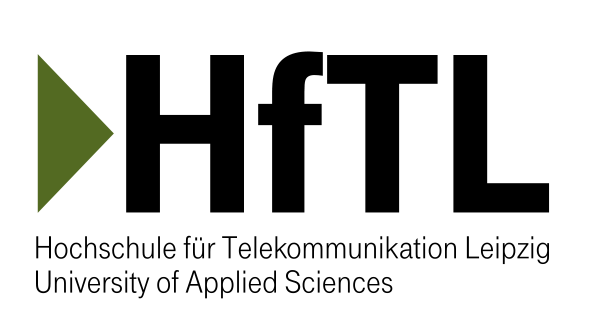
\includegraphics[width=2.5cm]{images/HfTL-Logo.png}
      \end{tabular}
      \hfill%
      \begin{tabular}[m]{c}
        Hochschule für Telekommunikation Leipzig (FH)\\
        Wirtschaftsinformatik \\
        Wissenschaftlich angeleitete Berufspraxis III\\
      \end{tabular}%
    }
  \end{center}
\end{figure}

\begin{center}
\rule{0pt}{0pt}
\vfill
\vfill
\vfill
\vfill

\begin{huge}
WAB III Projektarbeit:\\[0.75ex]
\dots\\[0.75ex]
E-Mail-Sicherheit\\[0.75ex]
\dots\\[0.75ex]
\end{huge}

\vfill
\vfill

Projektarbeit\\ von\\

\vspace*{.5cm}
Pascal Feller\\
Daniel Moy\\
Florian Schünhoff\\
Chi Cong Tran\\
\vspace{.5cm}
28. Juni 2014\\

\vfill
\vfill
\vfill
\vfill

\begin{tabular}{rl}
Referent, Betreuer:   & Prof. Dr. - Ing. Undine Pielot\\
\end{tabular}
\end{center}
\end{titlepage}



\newpage
\pagestyle{empty}


\text{ }
\vspace{11.5cm}




Hiermit versichern wir, dass wir die von uns vorgelegte Arbeit selbstständig verfasst haben, dass wir die verwendeten Quellen, Internet-Quellen und Hilfsmittel vollständig angegeben haben und dass wir die Stellen der Arbeit -- einschließlich Tabellen, Karten und Abbildungen~--, die anderen Werken oder dem Internet im Wortlaut oder dem Sinn nach entnommen sind, auf jeden Fall unter Angabe der Quelle als Entlehnung kenntlich gemacht haben.\\

Leipzig, den 28. Juni 2014\\
\medskip
\medskip

(Unterschrift)\\
\underline{~~~~~~~~~~~~~~~~~~~~~~~~~~~~~~~~~~~~~~~~}\\
Pascal Feller\\
\underline{~~~~~~~~~~~~~~~~~~~~~~~~~~~~~~~~~~~~~~~~}\\
Daniel Moy\\
\underline{~~~~~~~~~~~~~~~~~~~~~~~~~~~~~~~~~~~~~~~~}\\
Florian Schünhoff\\
\underline{~~~~~~~~~~~~~~~~~~~~~~~~~~~~~~~~~~~~~~~~}\\
Chi Cong Tran\\

\newpage


\pagestyle{empty}
%Seitenumbruch
\pagebreak

\pagenumbering{Roman}
%Inhaltsverzeichnis
\tableofcontents
\pagebreak
%Abbildungsverzeichnis
\listoffigures
\pagebreak
%falls ben�tigt auch noch ein Tabellenverzeichnis, m�sste dann die Auskommentierung aufgehoben werden
%\listoftables
%\pagebreak
%einbinden des in Akronyme.tex erstellten Abbildungsverzeichnisses
\phantomsection \addcontentsline{toc}{chapter}{Abkürzungsverzeichnis}
\renewcommand\refname{Abkürzungsverzeichnis} \chapter*{Abkürzungsverzeichnis}
\begin{acronym}[StuRa] % In die optionale eckige Klammer die längste Abkürzung schreiben (für gemeinsame Ausrichtung)
	\acro{DHE}{Diffie-Hellmann-Verfahren}
	\acro{TLS/SSL}{Transport Layer Security/Secure Socket Layer}
	\acro{PFS}{Perfect Foreward Secrecy}
\end{acronym}
\pagebreak

%�ndern der Seitennummerierung auf arabische Zahlen und Beginn bei Seite 1
\pagenumbering{arabic}\setcounter{page}{1}
%Dies ist die Vorlage für die einzelnen Kapitel, die jeweils mit Chapter als Kapiteltitel starten
\chapter{Titel des Kapitels}

%mit \section{title} wird ein Unterkapitel der ersten Gliederungsebene überschrieben
\section{Wichtiges Unterkapitel erster Gliederungsebene}
Lorem ipsum \dots

%mit \subsection{title} wird ein Unterkapitel der zweiten Gliederungsebene überschrieben
\subsection{Wichtiges Unterkapitel der zweiten Gliederungsebene}
Lorem ipsum \dots

%Vom Grundsatz war es das für die Erstellung von Kapiteln, jetzt kommt noch ein kleines Beispiel für Fußnoten
Dies ist ein großartiges Beispiel \footnote{Wenn einem nix einfällt muss man eben Quatsch schreiben} für eine Fußnote.
%Dies ist die Vorlage für die einzelnen Kapitel, die jeweils mit Chapter als Kapiteltitel starten
\chapter{Schlüsselaustausch}

%mit \section{title} wird ein Unterkapitel der ersten Gliederungsebene überschrieben
\section{Perfect Forward Secrecy - PFS}
%Problem
Beim klassischen Schlüsselaustausch werden die Sitzungsschlüssel durch den Public Key innerhalb des Server-Zertifikat übertragen.\footnote{Golem} Dies geschieht mittels RSA-Verfahren. Verschlüsselte Kommunikation ist jedoch nur solang die Schlüssel geheim bleiben sicher. Die Gefahr beim klassischen RSA-Public-Key-Verfahren ist dass vergangene Kommunikation nachträglich zu jedem Zeitpunkt entschlüsselt werden kann, sobald Angreifer in Besitz des Private Keys sind. 

%Idee
Sinnvoller ist es die Sitzungsschlüssel %REFERENZ Erklären was Sitzungsschlüssel sind
zum Einen nicht mehr zu übertragen und zum Anderen unabhängig voneinander ständig neu zu generieren und bei Terminierung zu löschen. 
Realisiert wird dies durch die Protokoll-Eigenschaft Forward Secrecy, die im Kryptographischen Fachjargon auch \ac{PFS}\footnote{golem} genannt wird.

%Umsetzung
Das \ac{DHE} ermöglicht die Aushandlung eines Sitzungsschlüssels bei dem die Kommunikationsparter verschiedene Nachrichten senden und sich auf einen Sitzungsschlüssel einigen können, ohne diesen je übertragen zu haben. Dieser Schlüssel ist auch nur für die aktuelle Verbindung gültig und wird anschließend gelöscht. Der Public-Key des Servers wird weiterhin übertragen, jedoch nur um den Schlüsselaustausch zu signieren. Die Verschlüsselungsverfahren \ac{TLS/SSL} und IPsec beherrschen bereits \ac{PFS}.

%Vorteile
Aufgezeichnete verschlüsselte Daten können somit bei Besitz des privaten Schlüssels nicht entschlüsselt werden. Zudem wird einfaches Belauschen einer aktiven Verbindung deutlich erschwert, denn es müsste die gesamte Kommunikation mit einem gezieltem Man-in-the-Middle Angriff manipuliert werden. Für diese Problematik gibt es wiederum moderne Ansätze wie DANE, die in Kombination mit PFS aktuell bei der Verschlüsselung von Verbindungen höchsten Sicherheitsansprüchen entsprechen, indem zusätzlich die Authentizät der Kommunikation gewährleistet wird. %REFERENZ MitM erklären 

%Nachteile
Nachteile gibt es lediglich bei der Verwendung des bereits überholten, und seit Jahren als geknackt bekannte DHE-Verfahren, denn dabei verzögert sich zusätzlich der Verbindungaufbau. Die Moduluslänge der Schlüssel ist Minimum 1024 Bit, und längere Schlüssel mit 2048 oder 4096 Bit sind debi nicht sicher. Der moderne Nachfolger mit elliptischen Kurven (ECDHE) gilt aktuell als sicher und benötigt dabei weniger als 1024 Bit und verzögert den Verbindungsaufbau nur unweigerlich. 

%Grenzen
Obwohl es Forward Secrecy bereits seit 1999 im TLS Standard 1.0 \footnote{golem} vorgesehen ist und smoit essenzieller Bestandteil von Verschlüsselung ist, hat sich PFS nocht nicht als Standard durchgesetzt.\footnote{https://www.trustworthyinternet.org/ssl-pulse/} Dies liegt zum einen an den Webservern. Mit einem Apache Webserver ist nur eine Moduluslänge von 1024 Bit vorgesehen. Beim Einsatz von DHE würden Provider damit ihre Server also unsicher betreiben. Zum Anderen sind es auf Client-Seite die Browser die noch nicht mitspielen. Der InternetExplorer verschlüsselt nur nach DSS, wobei der de-facto Standard für verschlüsselung RSA ist. Opera unterstützt lediglich das überholte DHE-Verfahren und Safari priorisiert Forward Secrecy niedrig und bevorzugt bei gegebener Option sogar die unverschlüsselte Kommunikation. Lediglich Firefox und Chrome unterstützen PFS in volle Umfang. 

%Browser prüfen und mit eigenen Quellen versehen

An dieser Stelle kann dann mal probiert werden ob Flaschenhals jetzt korrekt getrennt wird in dem ganz oft Flaschenhals geschrieben wird: Flaschenhals Flaschenhals Flaschenhals Flaschenhals Flaschenhals Flaschenhals Flaschenhals Flaschenhals Flaschenhals Flaschenhals
%Wenn automatisch erzeugtes Literaturverzeichnis verwendet wird, wird es hier eingef�gt
%\printbibliography
\end{document}